\documentclass{article}

\usepackage{amsmath}
\usepackage{amsthm}
\usepackage{amssymb}
\usepackage{amsfonts}
\usepackage[margin=0.5in]{geometry}
\usepackage[utf8]{inputenc}
\usepackage[spanish, mexico]{babel}
\usepackage{graphicx}

\title{Taller 5}
\author{Leidy Catherine Sánchez, Miguel Angel Gómez}

\begin{document}
	\maketitle
\paragraph{1.}Proof that.
$$a_0 + \frac{1}{2} \sum_{n=1}^{\infty} (a_n^2 + b_n^2) \leq \frac{1}{2T} \int_{-T}^{T} f(x)^2 dx.$$
\paragraph{}Known as the Bessel's inequality.
\begin{center}
	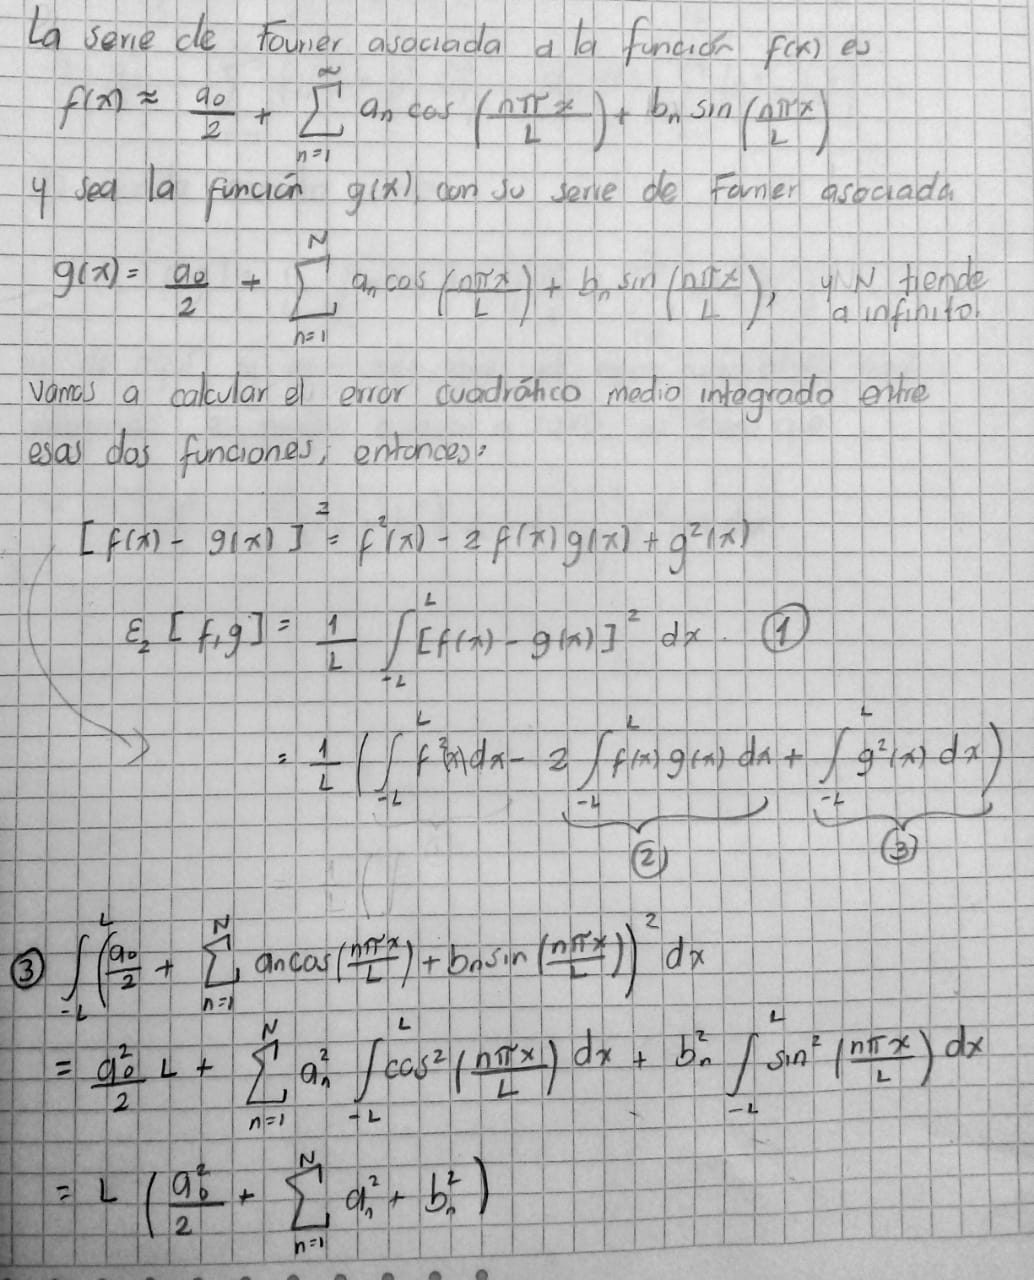
\includegraphics[width=0.5\textwidth]{img/1.jpeg}
\end{center}
\paragraph{2.} Write in full detail the proof, of Dirichlet theorem for Fourier series sketched in class.
\begin{center}
	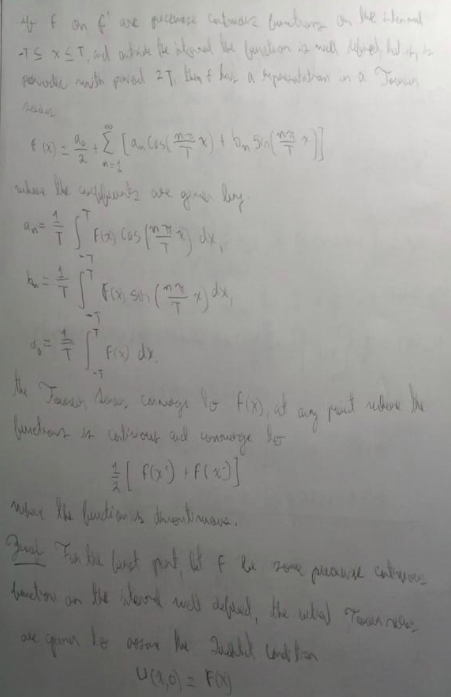
\includegraphics[width=0.7\textwidth]{img/2-1-1.png}
\end{center}
\begin{center}
	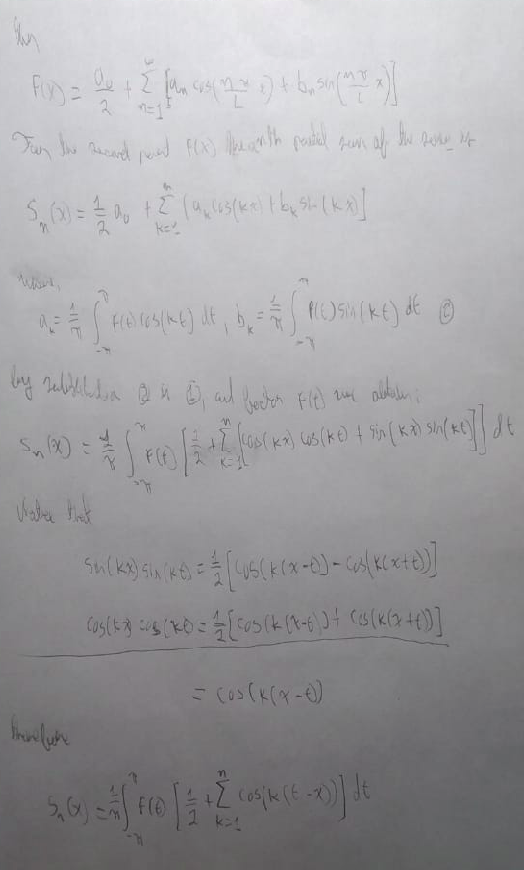
\includegraphics[width=0.7\textwidth]{img/2-1-2.png}
\end{center}
\begin{center}
	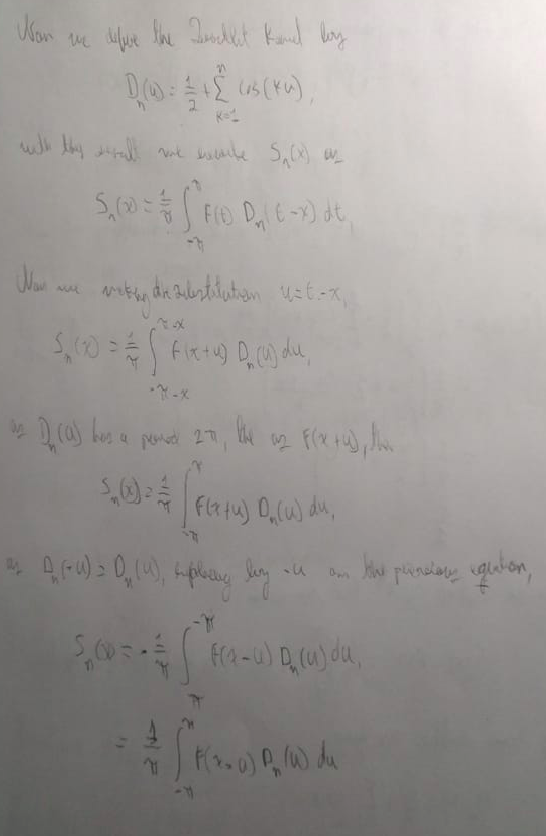
\includegraphics[width=0.7\textwidth]{img/2-1-3.png}
\end{center}
\begin{center}
	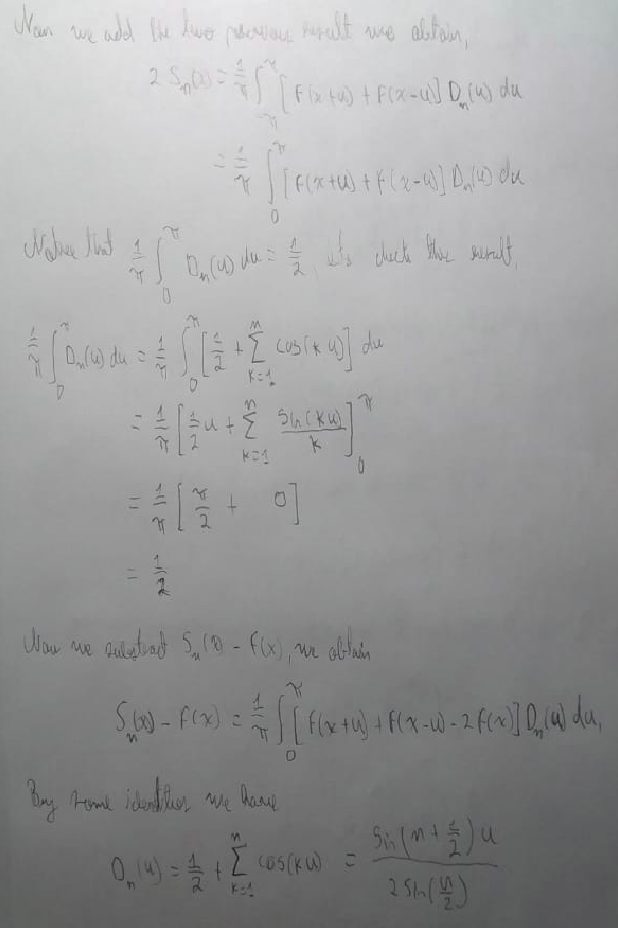
\includegraphics[width=0.7\textwidth]{img/2-1-4.png}
\end{center}
\begin{center}
	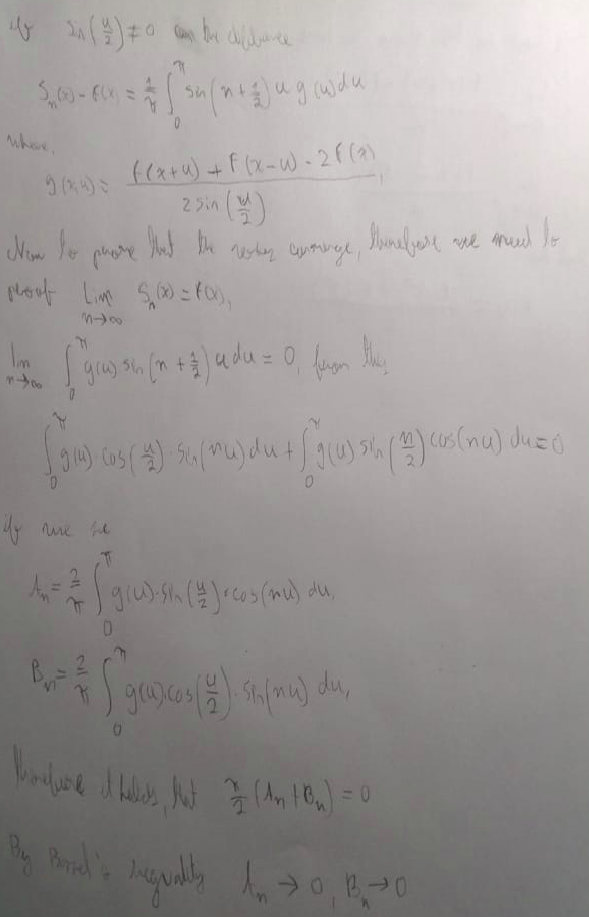
\includegraphics[width=0.7\textwidth]{img/2-1-5.png}
\end{center}
\begin{center}
	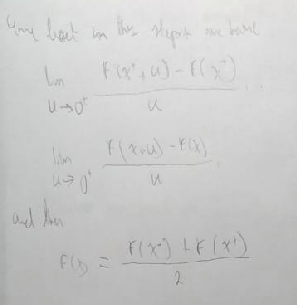
\includegraphics[width=0.7\textwidth]{img/2-1-6.png}
\end{center}
\newpage
\paragraph{3}.
\begin{center}
	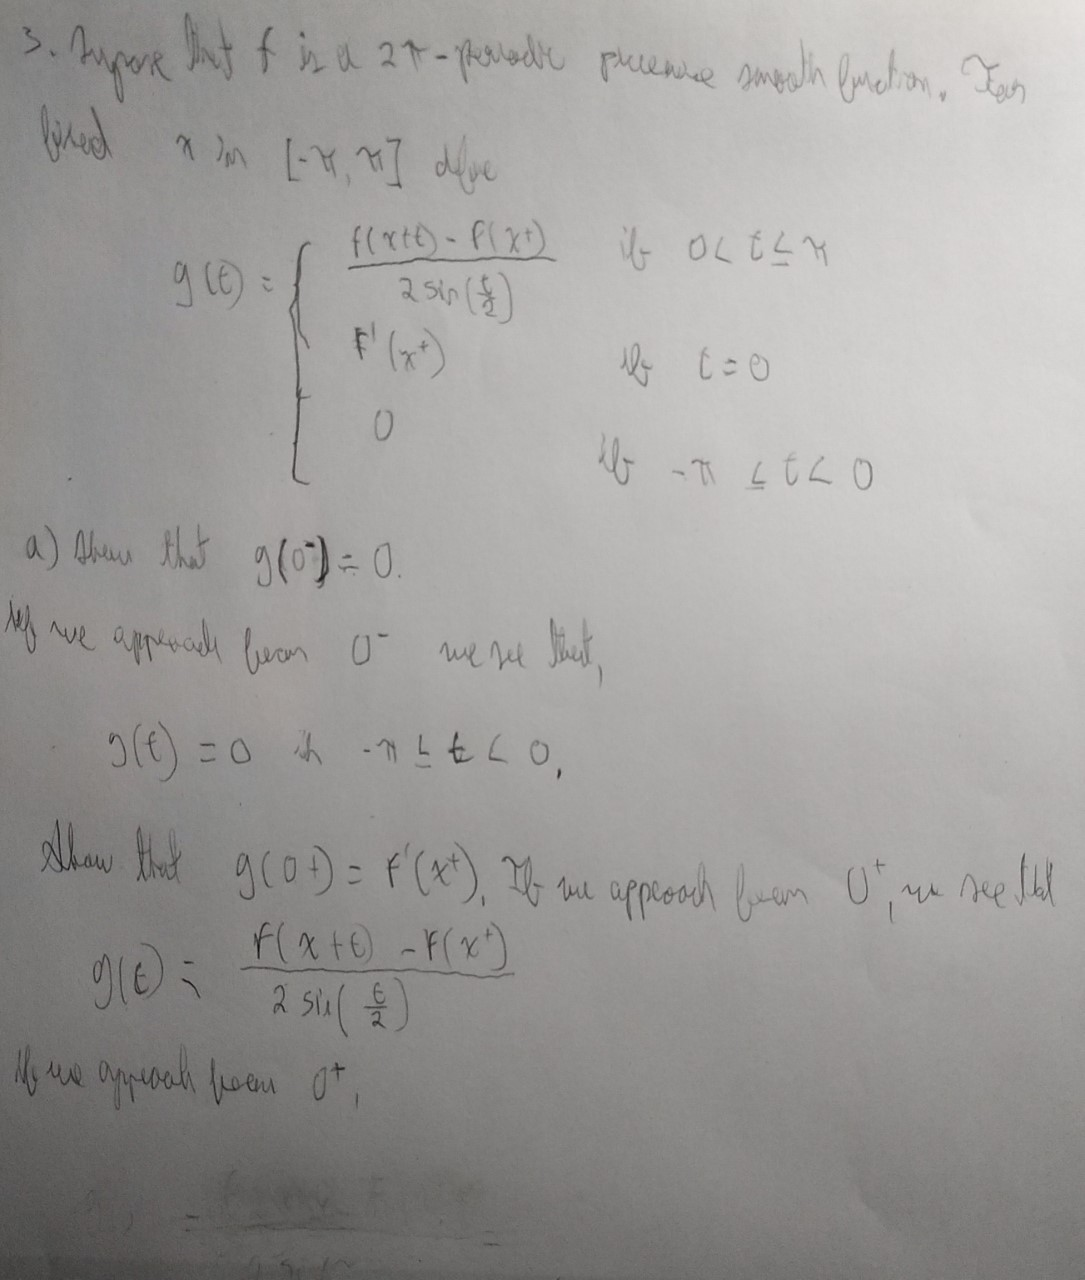
\includegraphics[width=0.7\textwidth]{img/3-1-a.jpg}
\end{center}
\newpage
\paragraph{4.}Prove the Parseval identity
$$\frac{1}{2T}\int_{T}^{T} f(x)^2 dx = a_0^2 + \frac{1}{2} \sum_{n=1}^{\infty} (a_n^2 + b_n^2)$$
\begin{center}
	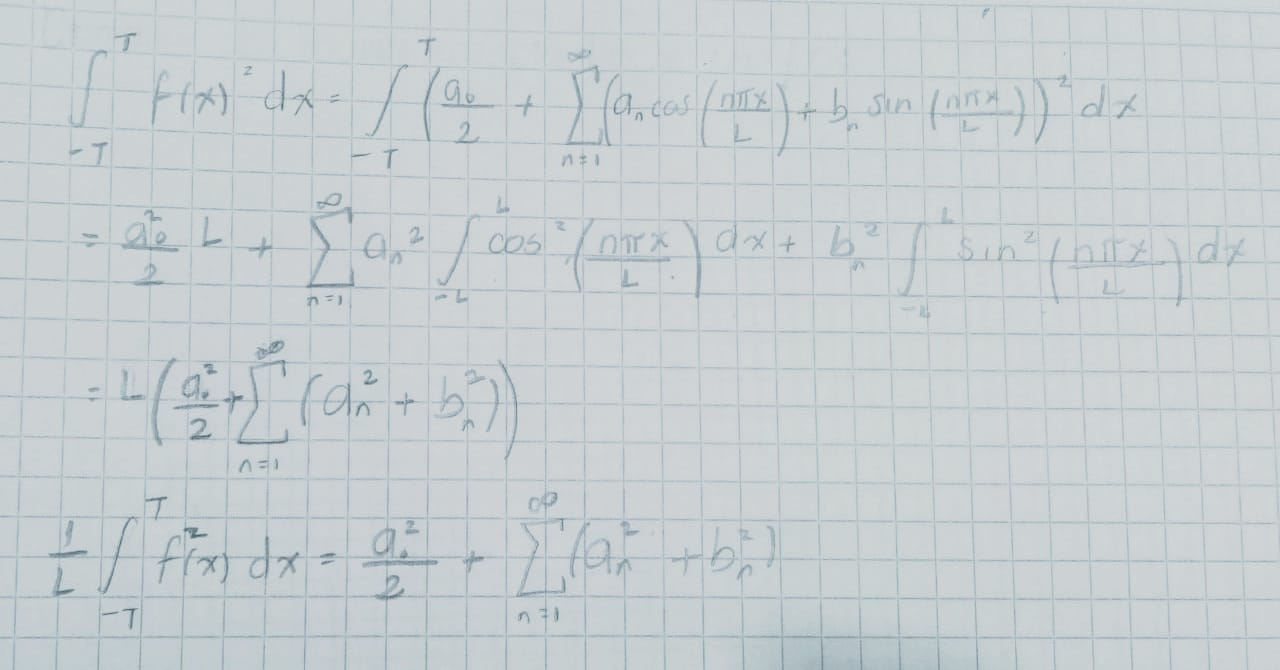
\includegraphics[width=0.7\textwidth]{img/4-1.jpeg}
\end{center}
\begin{center}
	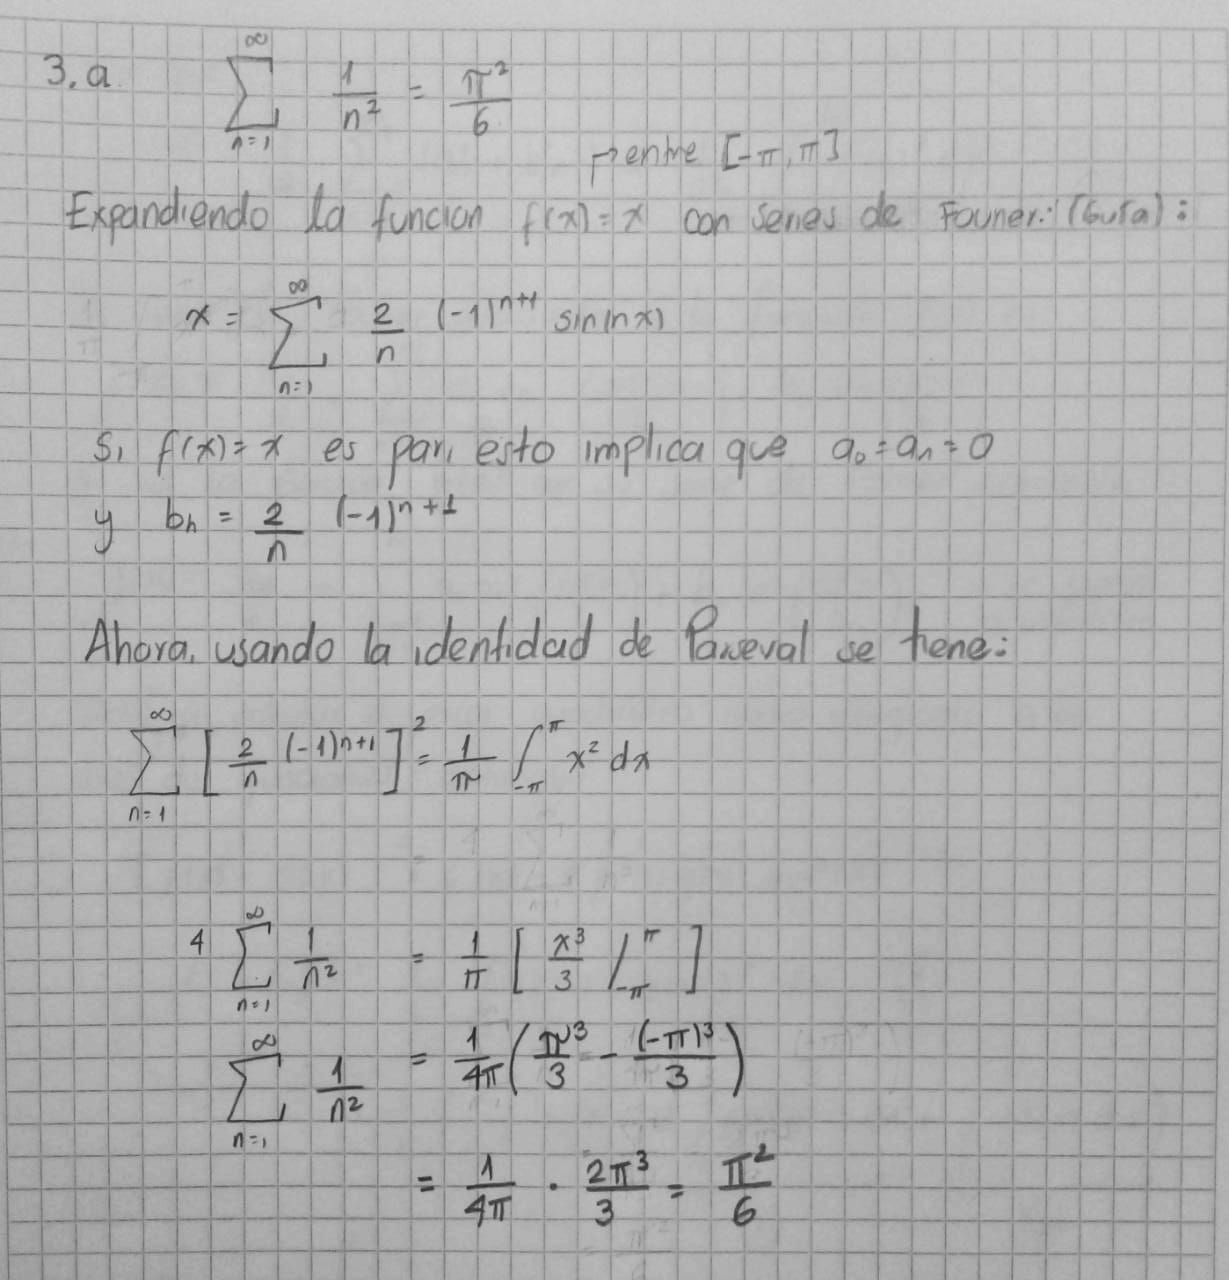
\includegraphics[width=0.7\textwidth]{img/4-2.jpeg}
\end{center}
\newpage
\begin{center}
	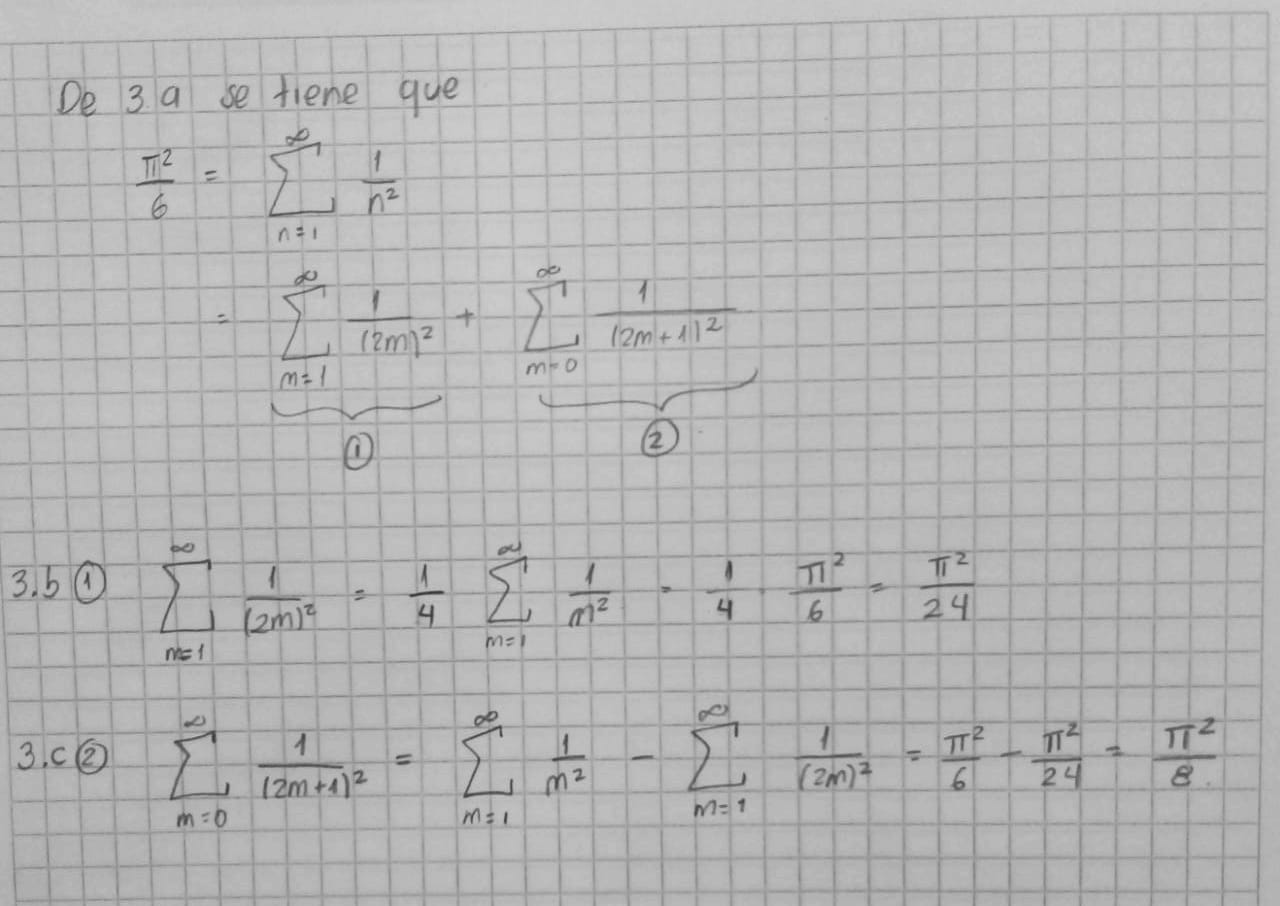
\includegraphics[width=0.7\textwidth]{img/4-3.jpeg}
\end{center}
\newpage
\paragraph{5.}
\begin{center}
	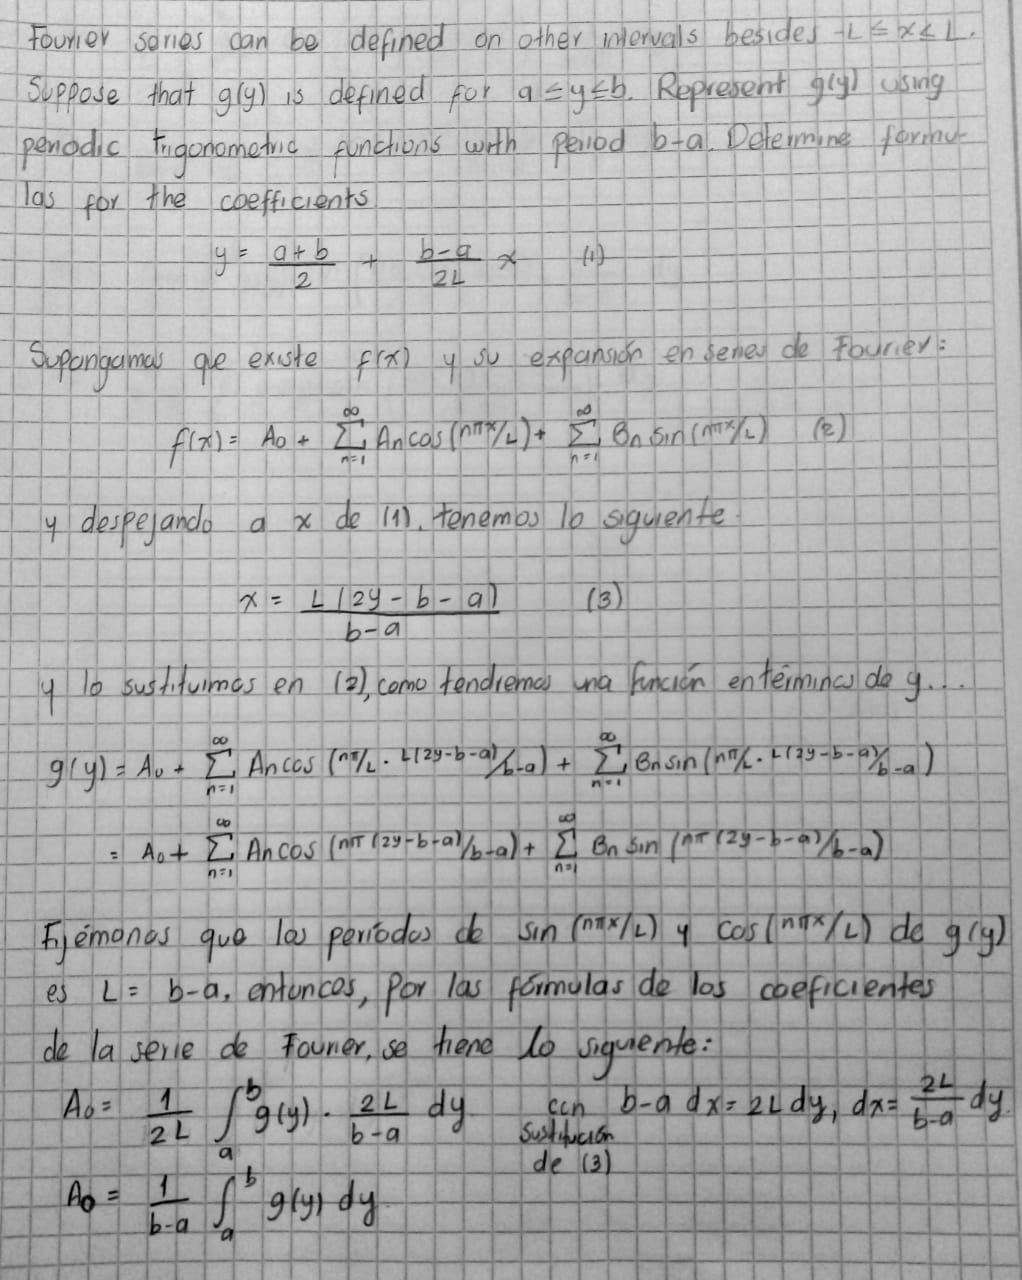
\includegraphics[width=0.7\textwidth]{img/5.jpeg}
\end{center}
\begin{center}
	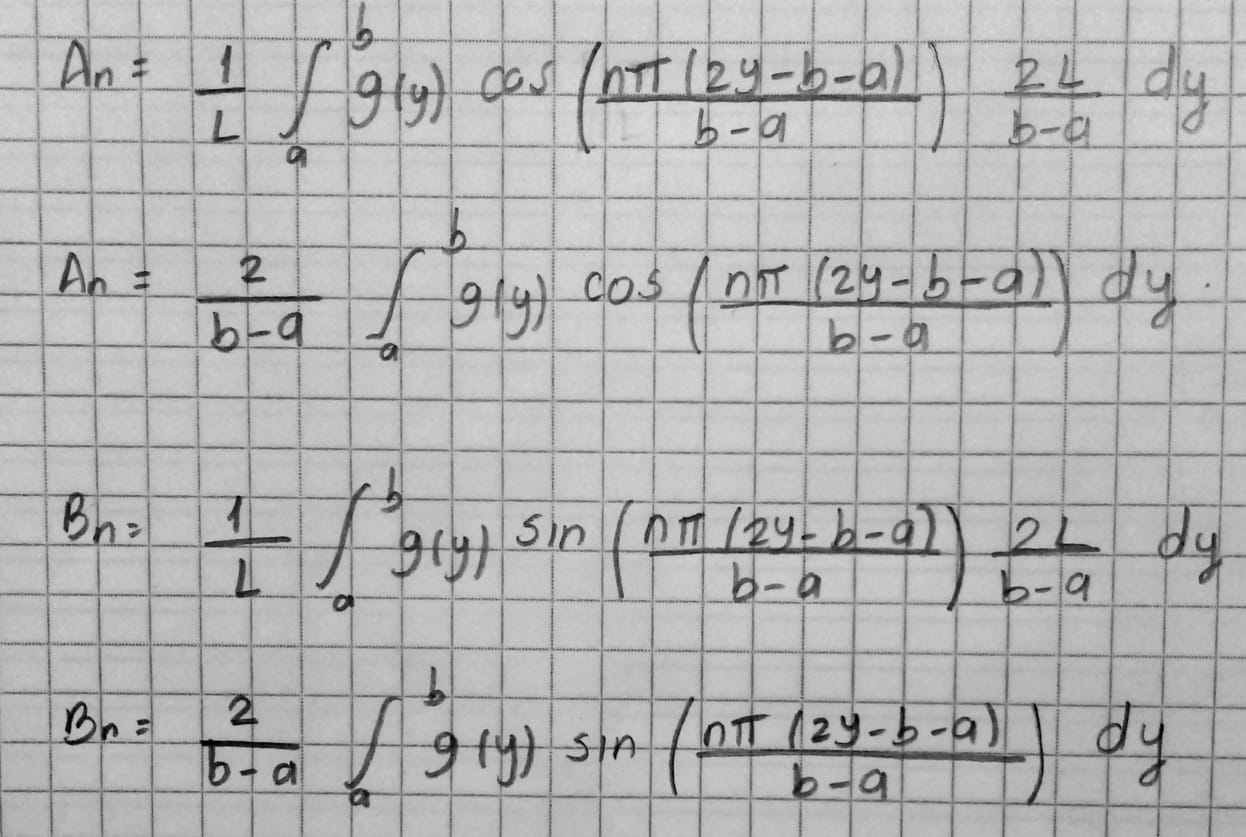
\includegraphics[width=0.7\textwidth]{img/5-2.jpeg}
\end{center}

\end{document}